%*****************************************
\chapter{Related Work}\label{ch:related_work}
%*****************************************
This chapter describes the related literature in the field of Cloud Computing Monitoring. Additional, this chapter provides a small overview of several state-of-the-art Open Source solutions that are relevant in developing a monitoring Cloud application. However, this chapter starts with a concise overview of related background material.

\section{Background} \label{sec:background}
This section provides background information for Cloud Computing Monitoring. Additionally, this section provides relevant challenges. Monitoring for the Cloud Consumer is primarily performed for discovering whether the service is working as expected. Additionally, Cloud Consumer Monitoring can be used for comparing monitoring data, from equivalent services, to decide which is the best one. However, it is important that the quality of the collected data is of a certain standard. The next section evaluates several properties of assessing this quality.

\subsection{Quality of data} \label{sec:quality}
The aspects for assessing the monitoring data quality are defined in \cite{wand1996anchoring}:
\begin{itemize}
    \item \textbf{Timeless: }the delay between a change of the real-world state and the resulting modification of the information system state.
    \item \textbf{Accuracy: }this implies that the information system represents a real-world state equivalent to the one that is represented.
    \item \textbf{Completeness: }the ability of an information system to represent every meaningful state of the represented real-world system.
    \item \textbf{Availability: }the extent to which data is present obtainable, and ready for use.
\end{itemize}

\noindent
Obtaining a good level of quality for the monitoring data according to these attributes depends on many factors. The monitoring system needs to be able to read the status of the attribute and to convert it into a value. There might be errors arising due to the precision of the data, the approximations done during the computations and the reliability of the formulas adopted. A proper balance between the cost of designing and running the monitoring system and the quality of the monitoring data is therefore crucial \cite{pernici2016monitoring}. 


\subsection{Open issues} \label{sec:open_issues}
In this section, several open issues and challenges are discussed. As stated in \cite{pernici2016monitoring, aceto2013cloud} there are multiple main issues in a systematic approach to monitoring. There are all described below.\\

\noindent
The first open issue is with respect to the specification of monitoring elements. It can be stated as: ``what monitoring data should be collected?'' The interesting data depends on the service being provided, and is thus different for every situation. Not only the elements to be monitored should be specified, but also the available sources. Another issue concerns the possibility of viewing the data and analysing it at different granularities. A third issue concerns the quality of the monitoring data, as can be evaluated by using the properties from \autoref{sec:quality}. Concerning sources, the monitoring system should be able to dynamically create or use new sources, in particular in services being provided in very variable situations, such as the ability to auto-scale in Docker\footnote{This is explained further in \autoref{sec:docker}.}\\

\noindent
Another open issue is concerned with the usage of the monitoring data. As there is variability in systems being monitored, there is also variability in the monitoring system behaviour. In some situations, monitoring is not always necessary or only a light observation is needed. In other situations, such as start up phases, there is stronger need for monitoring. In general, there is need to design the monitoring process. This can be done by specifying the requirements, related to different types of risks. The requirements include the specification of the quality parameters for monitoring elements, as described in \autoref{sec:quality}. Thus, there is a need to coordinate monitoring activities, and to investigate monitoring as a process. The specification of monitoring requirements needs additional research by designing formal models and methods.\\

\noindent
In \cite{aceto2013cloud} it is also stated that one of the open issues is the lack of custom algorithms and techniques that provide effective summaries. This paper also states the importance of accurate measures in an environment dominated by virtualized resources. Additionally, \cite{aceto2013cloud} argues that there are main improvements expected in terms of efficiency for data management. In particular, algorithms and techniques that are more efficient are needed to manage the large volume of monitoring data necessary to have a comprehensive view of the Cloud, in a way that is quickly and continuously.\\

\noindent
The complex structure of Cloud is made of several layers to allow for functional separation, modularity and thus manageable. However, such strong layering poses several limits on the monitoring system, in terms of kinds of analysis and consequent actions that can be performed. Therefore, another open research direction is to investigate possibilities of cross-layer monitoring.

\subsection{Conclusion}
This background section can be concluded with the fact that there are multiple open issues in the field of Cloud Computing Monitoring. When investigating methods that overcome one of these issues, it is important to keep the following two questions in mind:
\begin{itemize}
    \item What monitoring data should be collected?
    \item How can the monitoring data be used?
\end{itemize} 
The first question can be used to determine the monitoring data. This data needs to be evaluated according to the properties from \autoref{sec:quality}. Then, the second question can be answered. The final developed method must have validated both questions.


\section{Related literature} \label{sec:related_literature}
The research that is described in this thesis is the successor of the work performed by Ashton D. Spina. In \cite{spina} he explains the concern for the lack of non-proprietary tools to monitor cost and waste in a generalized manner on cloud deployments in the Virtual Machine as a Service (VMaaS) delivery model. He then proposes a general solution based on a set of probes (one per Virtual Machine), together with an aggregator. These tools are based on a set of requirements that describe the problem space. Although Spina has successfully shown that a monitoring solution that meets the elicited requirements can and has been created, there is future work to ensure quality of the tool. These improvements are mainly based to make the solution to be more effective and to be more user friendly. This section summarises several relevant papers. The papers are categorized by their main contribution. The following categories are evaluated: resource selection, monitoring architecture and estimating cost.

\subsection{Resource selection} \label{sec:resource_selection}
In \cite{wang2018self}, a description is provided that states the problem of monitoring cloud computing systems, as they are always in large scales and have complex architectures. To track the running status of these systems, a monitoring system always acquires kinds of monitoring data from different layers (e.g. network, hardware, virtual machine, operating system, middle-ware, application) in lots of distributed nodes. However, collecting, storing and processing a large amount of monitoring data should cause a huge resource overhead, which affects the timeliness of anomaly detection, the accuracy of fault locations, and even overall performance. Therefore, this paper proposes a self-adaptive monitoring framework. According to them, a distributed monitoring system needs to collect the following four key monitoring metrics:
\begin{itemize}
    \item \textbf{CPU: }CPU time occupied by system calls;
    \item \textbf{Network: }Number of packets received and sent;
    \item \textbf{Memory: }Number of bytes transferred from disk to memory;
    \item \textbf{Disk: }Number of bytes read and written;
\end{itemize}

\noindent
Using the collected metrics above, they must be represented in a statistical model. \cite{hauser2018reviewing} explains the representation of resource statistics. This statistical model consists of two parts: a state change probability matrix as the dynamic part, while a static part contains fixed information like CPU cores, and reference values of the underlying hardware for hardware independent comparisons. It presents an approach for monitoring resource statistics on the physical level only, and provide resource utilization profiles to cloud middle-ware and customers, instead of storing the raw time series data. Thus, its main advantage is the new approach of Cloud resource profiling by revisiting the necessary metrics for hardware independent resource profiles. This profile is interested for this research as it provides a critical view of the relevant resources that can be collected for monitoring cloud applications.\\


\noindent
According to \cite{aktas2018hybrid}, an important requirement in resource monitoring of cloud computing platforms is to monitor malfunctioning problems and/or security-related problems. Therefore, the detection of such problems becomes a highly important requirement for the continuous availability and maintenance of cloud computing systems. This paper presents a generic software architecture that is independent of the implementation of cloud computing platforms. The architecture is designed to provide two main functionalities for monitoring cloud computing platforms, i.e. (1) real-time monitoring for preventive maintenance and (2) after-the-fact monitoring for detecting malfunctions/security-related problems.\\

\subsection{Monitoring architecture} \label{sec:monitoring_architecture}
Parallel to the decision that needs to be made on what to monitor (i.e. which resource metrics, as described in \autoref{sec:resource_selection}), is to state how this can be achieved. This mainly concerns the architecture of the monitoring system. According to \cite{kumar2017inspection}, this can either be done centralized or decentralized. A centralized architecture has various issues, such as: (1) single point of failure, (2) not scalable, (3) high communication cost, and (4) lacking computational power. The authors of this paper argues for a decentralized architecture, which tackles the 4 issues described above. A monitoring system is considered decentralized when there is not a single component that is more necessary than another component.\\

\noindent
The authors from \cite{aktas2018hybrid} propose a generic software architecture that is independent of the implementations of cloud computing platforms. The architecture is designed to provide real-time monitoring and after-the-fact monitoring for detecting malfunctions/security-related problems. This decentralized system is implemented using the following components, a data collector, a message bus, a Distributed Stream Processing and Complex Event Processing Manager Modules, the preventive maintenance module, and an error detection module. They generated several tests and verified the proposed system against an increasing load. The prototype application is capable of processing a large volume of events in real-time detection capability for possible patterns that may lead to failures in VMs.\\

Equivalent to \cite{aktas2018hybrid}, is the development of another monitoring architecture that offers a monitoring platform-as-a-Service to each cloud consumer that allows to customize the monitoring metrics \cite{calero2014monpaas}. This is accomplished by means of an adaptive distributed monitoring architecture automatically deployed in the cloud infrastructure. The architecture has been implemented and released under GPL licence to the community as ``MonPaaS''. The architecture fulfils successfully all the requirements from the perspective of the Cloud Consumer:
\begin{itemize}
    \item Distributed architecture for high scalability.
    \item Allow cloud providers and consumers to monitor resources independently.
    \item Securely and privately provide monitoring information to the correct party.
    \item Disaster Recovery against failures.
    \item Discover automatically all the resources to be monitored (cold start).
    \item Allows cloud customer to extend, configure and customize the resources and services to be monitored (Monitoring-as-a-Service).
\end{itemize}

\subsection{Estimating cost} \label{sec:estimating_cost}
The last category that is relevant for this research is estimating the cost of deploying a Cloud Computing System. Various methods exist, such as Costradamus, which is described in \cite{kuhlenkamp2017costradamus}. This paper presents a generic cost model for cloud-based software services, and proposes metrics to quantify cost per API request. This model is based on one of the three possible tracing approaches: log import, response recording, and model-based tracing. Although this paper presents pricing models for popular public Cloud Providers, it lacks specificity when it comes to usage statistics and thus cost and waste of resources. This paper is more focussed on the utilization cost per request, instead of the utilization cost per (sub-)system.\\

\noindent
Another interesting paper on estimating deployment costs is \cite{leitner2016modelling}. It proses a method in which the total deployment cost is calculated as the sum of the costs of each individual service. The three primary drivers of service costs are the processing of domain functionality that the service is implementing, how many requests per time period it needs to accommodate, and in which quality (e.g., response time). Fundamentally, this model takes into account four cost factors: (1)compute costs (payment for the CPU time necessary to process service requests), (2) costs of API calls (per-request payment for each API call),  (3)costs of IO operations (payment for database or file system writes), and (4) costs of
additional options(e.g., payment for elastic IP addresses. These four key factors are important in this thesis for estimating the price of a deployment system.

\subsection{Conclusion} \label{sec:related_literature_conclusion}
The three categories are all relevant for the work in this thesis. For the resource selection, it can be concluded that four key monitoring metrics are necessary. Additional metrics can either be collected statistically, or dynamically. The last paper presents that real-time monitoring and after-the-factor monitoring are both necessary for detecting malfunctions. For the monitoring architecture, the decentralized architecture provides better scalability than the centralized equivalent. Lastly, for estimating the costs of deploying a Cloud Computing System, there lacks appropriate methods, and thus this needs to be developed in this research. 



\section{Related technologies} \label{sc:related_technologies}
Relevant technologies for the research in this thesis are cAdvisor, Prometheus and Grafana. This is a well known combination for resource monitoring, with the advantage that these three are all popular Open Source projects. Alternatives for this profiling stack are solutions like Nagios\footnote{\url{https://www.nagios.org/}}, Sensu\footnote{\url{https://sensu.io/}}, and New Relic\footnote{\url{https://newrelic.com/}} but they are too heavy and too expensive – or both. In the sections below, a description of each component is provided, together with their advantages.

\subsection{cAdvisor}
CAdvisor is hosted on Github\footnote{\url{https://github.com/google/cadvisor}} and aims to provide container users an understanding of the resource usage and performance characteristics of their running containers. It is a running daemon that collects, aggregates, processes, and exports information about running containers. Specifically, for each container it keeps resource isolation parameters, historical resource usage, histograms of complete historical resource usage and network statistics. This data is exported by container and machine-wide. The collected statistics are both exposed using their remote REST API, or can be scraped by Prometheus.

\subsection{Prometheus} 
Prometheus\footnote{\url{https://github.com/prometheus/prometheus/}} is a system originally developed by SoundCloud as part of a move towards a microservice architecture. It is a Time Series Database (TSDB) and a subset of its main features as compared to other monitoring systems are: 

\begin{itemize}
    \item A multi-dimensional data model (timeseries defined by metric name and set of key/value dimensions);
    \item A flexible query language to leverage this dimensionality;
    \item Timeseries collection happens via a pull model over HTTP;
    \item Support for hierarchical and horizontal federation;
\end{itemize}
    
Its architecture is interesting as it provides a better understanding of the possibilities with Prometheus and how it works. This architecture can be found in \autoref{fig:prometheus_architecture}. In this image, it can be seen that Prometheus collects its metrics by scraping multiple targets (called a job), and it can even scrape other Prometheus servers (known as federation). From this architecture, it also becomes clear that Prometheus can be configured with Grafana for presenting its visualizations. This is described in the next section.\\

\begin{figure}
    \centering
    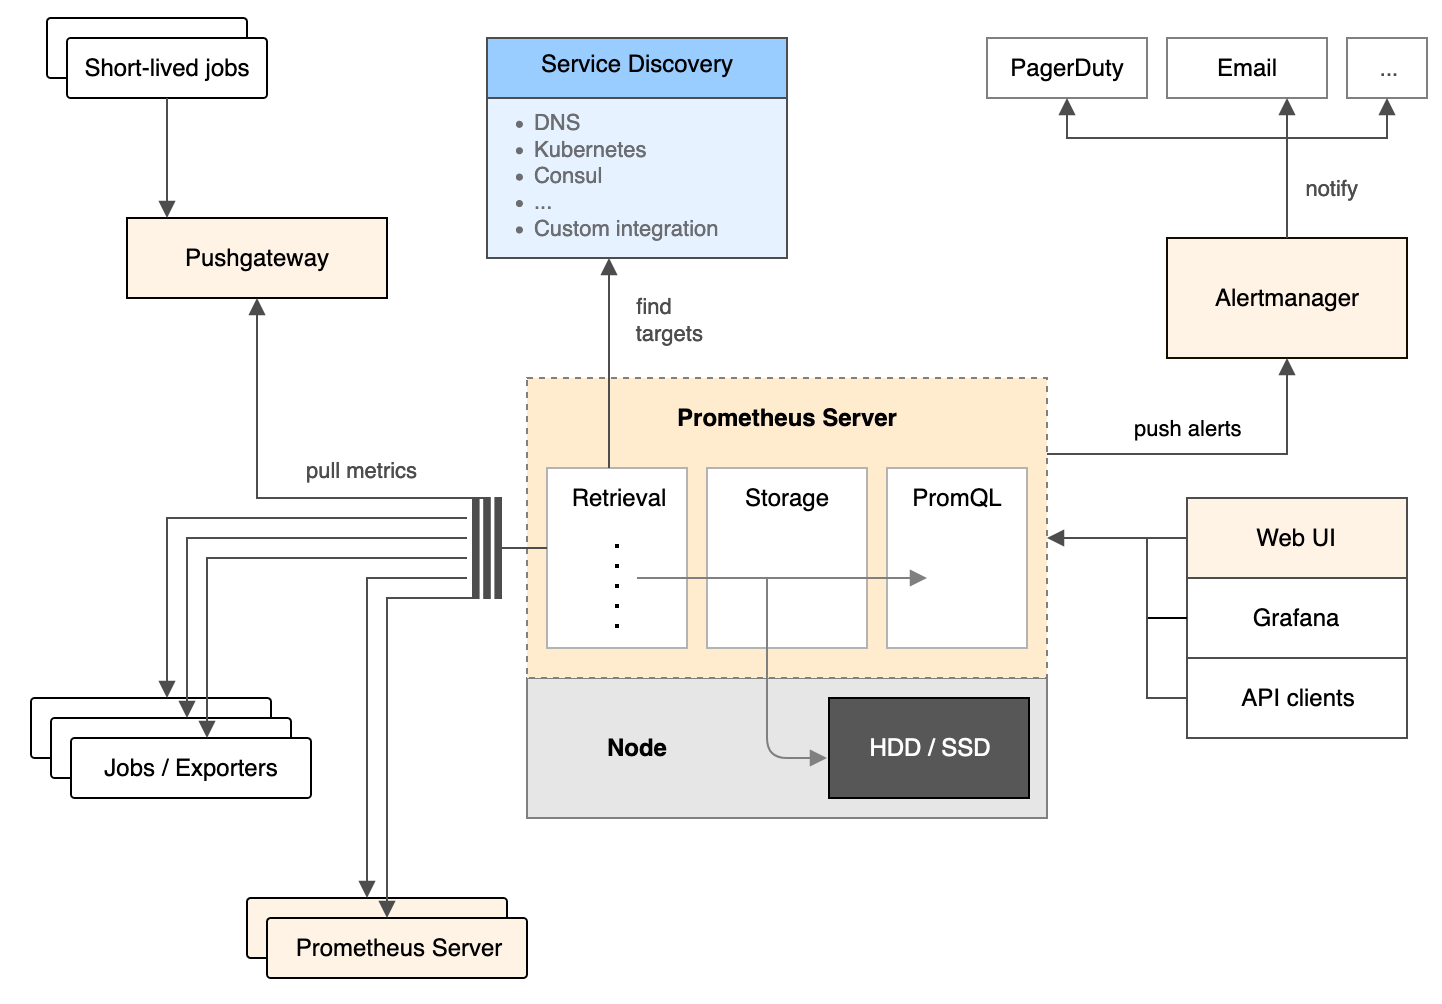
\includegraphics[width=\textwidth]{gfx/prometheus_architecture.png}
    \caption{Prometheus architecture}
    \label{fig:prometheus_architecture}
\end{figure}

Another interesting feature of Prometheus is how it represents its data. Unlike traditional SQL databases, the data is not structured in tables, rather it is structured as time series, in one of the four possible metric types \cite{prometheus_metrics}:
\begin{itemize}
    \item \textbf{Counter: }A counter is a cumulative metric that represents a single monotonically increasing counter whose value can only increase or be reset to zero on restart.
    \item \textbf{Gauge: }A gauge is a metric that represents a single numerical value that can arbitrarily go up and down.
    \item \textbf{Histogram: }A histogram samples observations (usually things like request durations or response sizes) and counts them in configurable buckets. It also provides a sum of all observed values.
    \item \textbf{Summary: }Similar to a histogram, a summary samples observations (usually things like request durations and response sizes). While it also provides a total count of observations and a sum of all observed values, it calculates configurable quantiles over a sliding time window.
\end{itemize}

\subsection{Grafana}
Grafana\footnote{\url{https://github.com/grafana/grafana}} allows you to query, visualize, alert on and understand your metrics no matter where they are stored. Grafana is highly customizable, which allows the user of Grafana to configure it to their needs. It can be configured to connect to different data sources, including Prometheus. Therefore, it is the perfect use for visualizing the results that are collected in this research. Grafana works with the notion of dashboards, which groups a set of visualizations together. A dashboard can be stored in a well known JSON format. A dashboard can be updated and configured by its graphical user interface. This results in an updated JSON file, which can be replaced by the original JSON dashboard. Therefore, it is straight forward to customize and configure the dashboard. A dashboard consists of several views, which are known as panels. There are already a set of predefined panels, including a graph, a heatmap, a pie chart, single stat (panel for displaying a single number) and a table. Every panel can be configured, so that it visualizes the required data. However, all visualizations are insufficient for this research, so a new one needs to be developed. This can be done by any language that compiles to Javascript. Therefore, the compiled source code results in the new panel. In Grafana, it is also possible to create an app, which is a combination of panels, data sources, dashboards and new UI pages. Apps can be imported directly in Grafana, so that there is no need for configuring anymore. 

\subsection{Docker} \label{sec:docker}
Docker is a technology that offers the ability to create, deploy, and run standardized software packages \cite{docker}. These software packages are known as containers, which can be created from images. Images specify how containers should operate and what software libraries are inside this container. Images are often created by combining and modifying standard images downloaded from public repositories, such as Dockerhub\footnote{\url{https://hub.docker.com/}}. Docker can be compared with a virtual machine, as they both offer some abstraction.  But unlike a virtual machine, rather than creating a whole virtual operating system, Docker allows applications to use the same Linux kernel as the system that it is running on and only requires applications be shipped with things not already running on the host computer. This gives a significant performance boost and reduces the size of the application.

\section{Discussion} \label{sec:relatedwork_discussion}

This chapter can be concluded with the fact that there are multiple open issues in the field of Cloud Computing Monitoring. These issues are with respect to the specification of monitoring elements, as well as the usage of the monitoring data. The research question proposed in \autoref{ch:research_question}



The first question can be used to determine the monitoring data. This data needs to be evaluated according to the properties from \autoref{sec:quality}. Then, the second question can be answered. The final developed method must have validated both questions.

The information described in the papers above highlight all another part of the requirements of developing a Cloud Computing Monitoring solution. Thus, \cite{wang2018self} explains the relevant metrics, \cite{aktas2018hybrid} explains a generic monitoring architecture, and \cite{hauser2018reviewing} explains a representation of resource statistics.